\begin{enunciado}{\ejExtra} {\tiny \violet{[segundo parcial 8/7/2023]}}
  Se sabe que cierto sistema físico que evoluciona con el tiempo cumple con el modelo $f(t) = a 2^{-2t} + b2^{-t}$ y se cuenta con la siguiente
  tabla con mediciones en el tiempo
  $$
    \begin{array}{|c||c|c|c|}
      \hline
      t    & 0  & 1 & 2   \\\hline
      f(t) & 10 & 3 & 3/4 \\\hline
    \end{array}
  $$
  Encontrar los valores $a$ y $b$ para que el modelo aproxime a los datos de la mejor forma en el sentido de cuadrados mínimos.
  ¿Los valores encontrados son únicos?
\end{enunciado}

Armar sistema matricial con los datos:
$$
  \llave{rcllllc}{
    f(0) & = &  10 & = & a2^{-2\cdot 0} + b 2^{-0} & = & a + b \\
    f(1) & = &   3 & = & a2^{-2\cdot 1} + b 2^{-1} & = & \frac{1}{4} a + \frac{1}{2}b \\
    f(2) & = &   \frac{3}{4} & = & a2^{-2\cdot 2} + b 2^{-2} & = & \frac{1}{16} a + \frac{1}{4} b
  }
  \flecha{forma}[matricial]
  A \vec{t} = \vec{f}(t)
  \sii
  \matriz{cc}{
    1 & 1 \\
    \frac{1}{4} & \frac{1}{2} \\
    \frac{1}{16} & \frac{1}{4}
  }
  \matriz{c}{
    a \\
    b
  }
  =
  \matriz{c}{
    10 \\
    3 \\
    \frac{3}{4}
  }
$$
Las ecuaciones normales:
$$
  A^tA \vec{f}(t) = A^t\vec{f}(t)
  \sii
  \matriz{cc}{
    \frac{273}{256} & \frac{73}{64} \\
    \frac{73}{64} & \frac{21}{16}
  }
  \matriz{c}{
    a \\
    b
  }
  =
  \matriz{c}{
    \frac{691}{64} \\
    \frac{187}{16}
  }
  \Sii{\red{!!}}
  \matriz{cc}{
    273 & 292 \\
    292 & 336
  }
  \matriz{c}{
    a \\
    b
  }
  =
  16
  \matriz{c}{
    \frac{691}{4} \\
    187
  }
  \sii
  \llave{rcl}{
    a \approx 8.51 \\
    b \approx 1.50
  }
$$
El modelo tiene solución única. La matriz del sistema $A$ tiene rango 2 y el sistema lineal a resolver tiene 2 parámetros $a$ y $b$.
$$
  \cajaResultado{
    f(t) = 8.51 \cdot 2^{-2t} + 1.5 \cdot 2^{-t}
  }
$$
Algo así, nada mal la verdad!
$$
  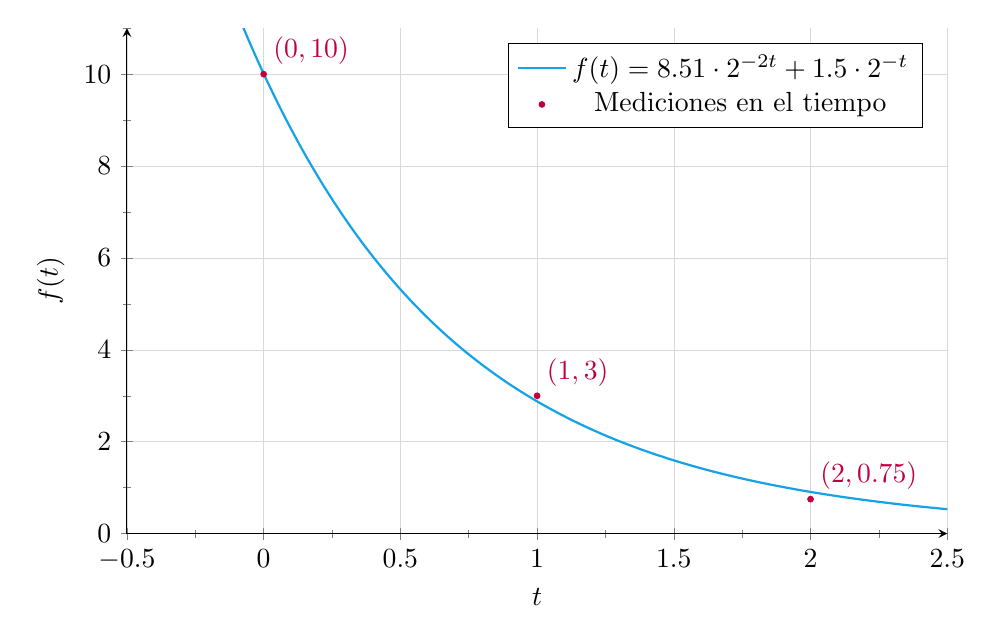
\begin{tikzpicture}
    \begin{axis}[
        axis lines = left,
        xlabel = {$t$},
        ylabel = {$f(t)$},
        xmin = -0.5, xmax = 2.5,
        ymin = 0, ymax = 11,
        grid = major,
        grid style = {very thin, gray!30},
        minor tick num = 1,
        minor grid style = {very thin, gray!15},
        width = 12cm,
        height = 8cm,
        samples = 200,
        smooth,
        legend pos = north east
      ]

      \addplot[
        domain=-0.5:2.5,
        Cerulean,
        thick
      ] {8.51 * 2^(-2*x) + 1.5 * 2^(-x)};
      \addlegendentry{$f(t) = 8.51 \cdot 2^{-2t} + 1.5 \cdot 2^{-t}$}

      \addplot[
        only marks,
        mark = *,
        mark size = 1pt,
        purple
      ] coordinates {
          (0, 10)
          (1, 3)
          (2, 0.75)
        };
      \addlegendentry{Mediciones en el tiempo}

      \node[above right, purple] at (axis cs:0,10) {$(0, 10)$};
      \node[above right, purple] at (axis cs:1,3) {$(1, 3)$};
      \node[above right, purple] at (axis cs:2,0.75) {$(2, 0.75)$};

    \end{axis}
  \end{tikzpicture}
$$

\begin{aportes}
  \item \aporte{\dirRepo}{naD GarRaz \github}
\end{aportes}
